\documentclass[../main.tex]{subfiles}

\begin{document}
\chapter{Stetige Funktionen}

\section{Stetigkeit}

Folgende Definition von Weierstrass
ist aus gutem Grund sehr berühmt.

\begin{definition}
  Sei $A \subset \mathbb{R}$ 
  eine beliebige Teilmenge.
  Eine Funktion
  $f \colon A \to \mathbb{R}$ 
  heisst \emph{stetig} im Punkt
  $p \in A$, falls für
  alle vorgegebenen $\varepsilon > 0$
  ein  $\delta > 0$ existiert,
  so dass für alle $q \in A$ 
  mit $|q-p| \leq \delta$ gilt,
  dass $|f(q) - f(p)| \leq \varepsilon$.
  Falls $f \colon A \to \mathbb{R}$ in
  allen Punkten $p \in A$ stetig ist,
  dann heisst $f$ \emph{stetig}.
\end{definition}

\begin{figure}[htb]
  \centering
  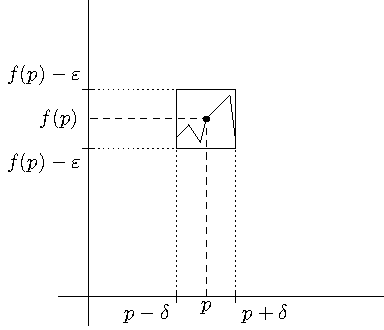
\includegraphics{images/conti}
  \caption{Stetigkeit bedeutet, dass der Graph
  der Funktion den Rand des eingezeichneten Rechtecks
nur rechts und links, aber nicht oben und unten
durchdringt.}%
  \label{fig:conti}
\end{figure}


\begin{examples}
  \leavevmode
  \begin{enumerate}[(1)]
    \item Die Identitätsfunktion
      \begin{align*}
        f \colon \mathbb{R} & \to \mathbb{R} \\
        p & \mapsto p
      \end{align*}
      ist stetig. Sei dazu $p \in \mathbb{R}$ fest
      und $\varepsilon > 0$ vorgegeben.
      Setze $\delta = \varepsilon$. Dann gilt
      für alle $q \in \mathbb{R}$ mit
      $|q - p| \leq \delta$, dass
      $|f(q) - f(p)| = |q - p| \leq \delta = \varepsilon$.
    \item Sei
      \[
        f(x) = 
        \begin{cases}
          0 & \text{falls } x \leq 0, \\
          1 & \text{falls } x > 0,
        \end{cases}
      \]
      siehe Abbildung~\ref{fig:jump}.
      Dann ist $f$ in allen Punkten ausser dem
      Nullpunkt stetig.
      Tatsächlich, sei $p \neq 0$
      und $\varepsilon > 0$ 
      vorgegeben.
      Setze $\delta = |p|/2 > 0$.
      Dann gilt für alle $q \in \mathbb{R}$ 
      mit $|q - p| \leq \delta$, dass
      $|f(q) - f(p)| = 0 \leq \varepsilon$.
      
      Sei nun $p = 0$. Betrachte $\varepsilon = 1/2$.
      Sei $\delta > 0$ beliebig.
      Dann gilt für $q = \delta/2$, dass
      $|q - p| = \delta/2 < \delta$.
      Es folgt
      \[
        |f(q) - f(p)| = |1 - 0| = 1 > \varepsilon.
      \]
      \begin{figure}[htb]
        \centering
      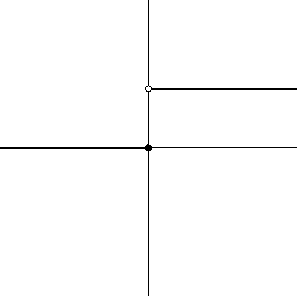
\includegraphics{images/jump}
        \caption{Sprungstelle}%
        \label{fig:jump}
      \end{figure}

    \item Sei
      \[
        f(x) = 
        \begin{cases}
          1, & \text{falls } x \in \mathbb{Q}, \\
        0,& \text{falls } x \in \mathbb{R} \setminus \mathbb{Q}
        \end{cases}
      \]
      die \emph{Dirichletfunktion}.
      Dann ist $f$ in keinem Punkt stetig.
      Betrachte dazu $\varepsilon = 1/2$.
      Sei $p \in \mathbb{Q}$, das heisst, $f(p) = 1$.
      Für alle $\delta > 0$ finden wir eine
      irrationale Zahl
      $q \in \mathbb{R} \setminus \mathbb{Q}$ mit
      $|q - p| \leq \delta$ 
      und
      $|f(q) - f(p)| = 1 > \varepsilon$.
      Tatsächlich, wähle $N \in \mathbb{N}$ 
      mit $\sqrt 2 / N \leq \delta$.
      Setze
      $q = p +\sqrt 2/N$. Dann gilt  $q \notin \mathbb{Q}$,
      also $f(q) = 0$.

      Analog, sei $p \in \mathbb{R} \setminus \mathbb{Q}$,
      das heisst, $f(p) = 0$.
      Für alle $\delta > 0$ finden wir
      eine Zahl $q \in \mathbb{Q}$ mit $|q - p| \leq \delta$ 
      und
      $|f(q) - f(p)| = 1 > \varepsilon$.
      Tatsächlich,
      wähle $N \in \mathbb{N}$ mit $1/N \leq \delta$.
      Dann existiert $a \in \mathbb{Z}$,
      so dass
      $|a/N - p| \leq 1/N$.
      Setze $q = a/N$.
    \item Sei $f(x) = x^n$ für $n \in \mathbb{N}$.
      Dann ist $f$ stetig auf $\mathbb{R}$.
      Sei also $p \in \mathbb{R}$ vorgegeben und
      sei $\varepsilon > 0$.
      Für
      $h \in \mathbb{R}$ mit $|h| \leq 1$ gilt
      \[
        f(x + h) = {(x + h)}^n = \sum_{k=0}^{n} \binom{n}{k}
        x^{n-k}h^k
        = x^n + nx^{n-1}h + \frac{n(n-1)}{2}x^{n-2}h^2 + \cdots.
      \]
      Es folgt, dass
      \[
        |f(x + h) - f(x)| \leq |h| \cdot
        \left| \sum_{k=1}^{n} \binom{n}{k} x^{n-k} \right|,
      \]
      da $|h| \leq 1$.
      Setze jetzt
      \[
        \delta_1 = \frac{\varepsilon}{t+1},
      \]
      wobei
      \[
        t = \sum_{k=1}^{n} \binom{n}{k} |p|^{n-k},
      \]
      und $\delta = \min \{1, \delta_1\} > 0$.
      Für alle  $h \in \mathbb{R}$
      mit $|h| \leq \delta$ gilt also
      \[
        |f(p+h) - f(p)| \leq |h| \cdot t \leq
        \delta_1 \cdot t = \varepsilon \cdot \frac{t}{t+1}
        \leq \varepsilon.
      \]
      Also ist $f$ stetig im Punkt $p$.
    \item Betrachte die Funktion
      \begin{align*}
        f \colon \mathbb{R} \setminus \{0\} & \to \mathbb{R} \\
        x & \mapsto 1/x.
      \end{align*}
      Dann ist $f$ stetig in allen Punkten
      $p \in \mathbb{R} \setminus \{0\}$. Dies ist
      mühsam von Hand zu zeigen. Deshalb
      verwenden wir folgendes Lemma.
  \end{enumerate}
\end{examples}

\begin{lemma*}
  Sei $A \subset \mathbb{R}$ und seien
  $f, g \colon A \to \mathbb{R}$ im Punkt
  $p \in A$ stetig. Dann sind die Funktionen
  $f + g$ und $f \cdot g$ 
  im Punkt $p$ stetig.
  Falls $f(p) \neq 0$, dann
  existiert $a > 0$, so dass
  die Funktion $1/f$ auf der Menge
  $(p- a, p + a) \cap A$ definiert und 
  im Punkt $p$ stetig ist.
\end{lemma*}

\begin{proof}
  Als erstes zeigen wir,
  dass $f  + g$ stetig ist.
  Sei $\varepsilon > 0$ vorgegeben.
  Wähle $\delta_f > 0$ und  $\delta_g > 0$ 
  so, dass für alle $q \in A$ mit
  $|q - p| \leq \delta_f$ gilt, dass
  $|f(q) - f(p)| \leq \varepsilon/2$,
  und so, dass für alle
  $q \in A$ mit $|q - p| \leq \delta_g$ 
  gilt, dass
  $|g(p) - g(q)| \leq \varepsilon/2$.
  Setze $\delta = \min \{\delta_f, \delta_g\}$.
  Dann gilt für alle $q \in A$ mit
  $|q - p| \leq \delta$, dass
  \begin{align*}
  |(f + g)(q) - (f + g)(p)| &     = |f(q) + g(q) - f(p) - g(p)|\\
                            & \leq |f(q) - f(p)| + |g(q) - g(p)|\\
                            & \leq \varepsilon/2 + \varepsilon/2\\
                            &= \varepsilon.
  \end{align*}

  Wir zeigen nun, dass $f \cdot g$ stetig ist.
  Berechne
  \begin{align*}
     |(f\cdot g)(q) - (f \cdot g)(p)|
     & = |f(q) \cdot g(q) - f(p) \cdot g(p)| \\
     & = |f(q)g(q) - f(p)g(q) + f(p)g(q) - f(p) g(p)| \\
     & \leq |g(q)| \cdot |f(q) - f(p)| + 
     |f(p)| \cdot |g(q) - g(p)|.
  \end{align*}
  Wähle $\delta_1 > 0$ so, dass immer wenn
  $|q - p| \leq \delta_1$ gilt, dann auch
  $|g(q) - g(p)| \leq 1$. Wähle
  $\delta_2 > 0$ so, dass immer
  wenn $|q - p| \leq \delta_2$ gilt, dann auch
  \[
    |f(q) - f(p)| \leq \frac{\varepsilon}{2} \cdot
    \frac{1}{|g(p)| + 1}.
  \]
  Wähle weiterhin $\delta_3 > 0$ so, dass immer wenn
  $|q - p| \leq \delta_3$ gilt, dann auch
  \[
    |g(q) - g(p)| \leq \frac{\varepsilon}{2} \cdot
    \frac{1}{|f(p)| + 1}.
  \]
  Setze $\delta = \min \{\delta_1, \delta_2, \delta_3 \}$.
  Für $q \in A$ mit $|q - p| \leq \delta$ gilt dann:
  \begin{align*}
    |(f \cdot g)(q) - (f \cdot g)(p)|
    &\leq |g(q)| \cdot \frac{\varepsilon}{2} \cdot  
    \frac{1}{|g(p)| + 1}
    + |f(p)| \cdot \frac{\varepsilon}{2}
    \cdot \frac{1}{|f(p)| + 1}\\
    & \leq (|g(p)| + 1) \frac{\varepsilon}{2}
    \cdot \frac{1}{|g(p)| + 1} + \frac{\varepsilon}{2}  \\
    &= \varepsilon.
  \end{align*}
  
  Zuletzt behandeln wir $1/f$.
  Sei $p \in A$ mit $f(p) \neq 0$.
  Dann existiert nach Stetigkeit von
  $f$ im Punkt $p$ eine Zahl $a > 0$, so dass
  wenn $|q - p| \leq a$ gilt,
  dann auch
  \[
  |f(q) - f(p)| \leq \frac{|f(p)|}{2}.
  \]
  Also ist $1/f$ auf der Menge $(p-a, p+a) \cap A$ definiert,
  da dort $|f(q)| \geq \frac{|f(p)|}{2} > 0$. % braucht man für Beweis
  Sei nun $\varepsilon > 0$. 
  Berechne
   \begin{align*}
     \left| \frac{1}{f(q)} - \frac{1}{f(p)} \right| 
     & = \left| \frac{f(p) - f(q)}{f(q)f(p)} \right| \\
     & \leq 2 \cdot \frac{|f(p) - f(q)|}{|f(p)|^2}. 
  \end{align*}
  Wähle $\delta > 0$ so, dass $\delta \leq a$ 
  und immer wenn $|q - p| \leq \delta$,
  dann auch 
  \[
    |f(q) - f(p)| \leq \frac{\varepsilon}{2} \cdot |f(p)|^2.
  \]
  Es folgt für $q \in A$ mit $|q - p| \leq \delta$, dass
  \[
    \left| \frac{1}{f(q)}- \frac{1}{f(p)} \right|
    \leq 2 \cdot \frac{|f(p) - f(q)|}{|f(p)|^2} \leq \varepsilon.
    \qedhere
  \]
\end{proof}

\begin{applications}
  \leavevmode
  \begin{enumerate}[(1)]
    \item Alle Funktionen der Form
      \[
        f(x) = a_n x^n + a_{n-1} x^{n-1} + \cdots + a_{1} x + a_0,
      \]
      sogenannte \emph{Polynome},
      mit Koeffizienten $a_k \in \mathbb{R}$ sind stetig
      auf $\mathbb{R}$, da die Identitätsfunktion $x \mapsto x$
      und konstante Funktionen stetig sind.
    \item Die Funktion $f(x) = 1/x$ ist stetig
      auf $\mathbb{R} \setminus \{0\}$.
  \end{enumerate}
\end{applications}

\subsection*{Folgenstetigkeit}
\begin{theorem}
  Sei $A \subset \mathbb{R}$ eine Teilmenge.
  Eine Funktion $f \colon A \to \mathbb{R}$ ist
  genau dann stetig im Punkt
  $p \in A$, wenn für alle
  konvergenten Folgen $a \colon \mathbb{N} \to A$
  mit $\lim_{n \to \infty}a_n = p \in A$ gilt, dass
  \[
    \lim_{n \to \infty} f(a_n) = f(p).
  \]
\end{theorem}

\begin{proof}
  Für die Hinrichtung ``$\Rightarrow$'' sei $f$
  im Punkt $p$ stetig. Sei ${(a_{n})}_{n \in \mathbb{N}}$ 
  eine Folge in $A$ mit
  \[
    \lim_{n \to \infty} a_n = p.
  \]
  Sei $\varepsilon > 0$ vorgegeben.
  Dann existiert $\delta > 0$, so dass immer wenn
  $|q - p| \leq \delta$, dann auch
  $|f(q) - f(p)| \leq \varepsilon$.
  Wähle $N \in \mathbb{N}$ so,
  dass für $n \in \mathbb{N}$ mit $n \geq N$ gilt,
  dass $|a_n - p| \leq \delta$.
  Es gilt also für $n \geq N$, dass
  $|f(a_n) - f(p)| \leq \varepsilon$.
  Also gilt
  \[
    \lim_{n \to \infty} f(a_n) = f(p).
  \]
  
  Für die Rückrichtung ``$\Leftarrow$'', nimm an,
  dass $f$ \emph{folgenstetig} in $p$ ist,
  das heisst, dass für alle
  konvergenten Folgen $a \colon \mathbb{N} \to A$
  mit $\lim_{n \to \infty} a_n = p$ gilt,
  dass
  \[
    \lim_{n \to \infty} f(a_n) = f(p).
  \]
  Wir beweisen durch Widerspruch, dass
  $f$ stetig in $p$ ist.
  Nimm an, dass $f$ nicht stetig in $p$ ist.
  Dann existiert $\varepsilon_0 > 0$, so dass
  für alle $\delta > 0$ ein $q \in A$ 
  existiert, so dass
  $|q - p| \leq \delta$ und $|f(q) - f(p)| > \varepsilon_0$.
  Wähle nun eine Folge
  ${(a_{n})}_{n \in \mathbb{N}}$ wie folgt.
  Wähle $a_n \in A$ so, dass
  $|a_n - p| \leq 1/(n+1)$ und $|f(a_n) - f(p)| > \varepsilon_0$.
  Nach Konstruktion gilt
  $\lim_{n \to \infty} a_n = p$, aber
  \[
    \lim_{n \to \infty} f(a_n) \neq f(p).
  \]
  Dies widerspricht der Folgenstetigkeit von $f$.
\end{proof}

Dieser Satz sagt, dass genau dann die Formel
\[
  \lim_{n \to \infty}  f(a_n) = f\left(\lim_{n \to \infty} a_n\right)
\]
für alle konvergenten Folgen ${(a_{n})}_{n \in \mathbb{N}}$ in $A$
mit Grenzwert in $A$
gilt, wenn $f$ stetig ist.

\begin{application}
  Seien $f \colon A \to \mathbb{R}$ und $g \colon B \to \mathbb{R}$
  Funktionen mit $f(A) \subset B$. Falls $f$ im Punkt $p \in A$ 
  stetig ist, und $g$ im Punkt $f(p) \in B$ stetig ist,
  dann ist $g \circ f\colon A \to \mathbb{R}$ im Punkt $p$ stetig.
\end{application}

\begin{proof}
  Wir verwenden die Folgenstetigkeit um einen schnellen
  Beweis zu liefern.
  Sei  ${(a_{n})}_{n \in \mathbb{N}}$ eine konvergente
  Folge in $A$ mit $\lim_{n \to \infty} a_n = p \in A$.
  Da $f$ stetig in $p$ ist, folgt
  \[
    \lim_{n \to \infty}f(a_n) = f(p).
  \]
  Setze $b_n = f(a_n)$. Dann ist ${(b_{n})}_{n \in \mathbb{N}}$ 
  eine konvergente Folge in $f(A) \subset B$ mit Grenzwert
  $f(p)$.
  Da $g$ stetig in $f(p)$ ist, folgt
  \[
    \lim_{n \to \infty} g(b_n) = g(f(p)).
  \]
  Wir folgern, dass
  \[
    \lim_{n \to \infty} (g \circ f)(a_n) = (g \circ f)(p),
  \]
  das heisst, $g \circ f$ ist stetig im Punkt $p$.
\end{proof}

\begin{example}
  Betrachte die stetigen Funktionen
  \begin{align*}
    f \colon \mathbb{R} & \to \mathbb{R} \\
    x & \mapsto x(x-1)
  \end{align*}
  und
  \begin{align*}
    g \colon \mathbb{R} \setminus \{0\} & \to \mathbb{R} \\
     x & \mapsto 1/x.
  \end{align*}
  Dann ist
  \[
    (g \circ f)(x) = \frac{1}{x(x-1)}
  \]
  stetig auf $\mathbb{R} \setminus \{0, 1\}$.
\end{example}


\begin{remark}
  Die Funktion $f(x) = 1/x$ hat keine
  stetige Fortsetzung auf $\mathbb{R}$,
  das heisst, es existiert keine stetige
  Funktion $\overline f \colon \mathbb{R} \to \mathbb{R}$,
  so dass $\overline f |_{\mathbb{R} \setminus \{0\}} = f$.
  Hier ist \[\overline f |_{\mathbb{R} \setminus\{0\}}
  \colon \mathbb{R} \setminus \{0\} \to \mathbb{R}\]
  die Funktion $\overline f$ \emph{eingeschränkt} auf
  $\mathbb{R} \setminus \{0\}$, 
  gegeben durch 
  $\overline f|_{\mathbb{R} \setminus \{0\}}(x) =f(x) $
  für $x \in \mathbb{R} \setminus \{0\}$.
\end{remark}

Es kann jedoch sein, dass für gewisse
Funktionen $g$ die Funktion
$g \circ f$ eine stetige Fortsetzung auf $\mathbb{R}$ hat.

\begin{examples}
  \leavevmode
  \begin{enumerate}[(1)]
    \item Sei $g \colon \mathbb{R} \to \mathbb{R}$ gegeben
      durch $g(x) = 0$ für alle $x$. Dann ist
      $g \circ f(x) = 0$ auf $\mathbb{R} \setminus \{0\}$,
      was eine stetige Fortsetzung (die konstante Nullfunktion)
      auf $\mathbb{R}$ hat.
    \item Sei $g(x) = 1/x$ auf $\mathbb{R} \setminus \{0\}$.
      Dann hat $g \circ f(x)$ auf $\mathbb{R}$ 
      eine stetige Fortsetzung (die Identitätsfunktion $x
      \mapsto x$) auf $\mathbb{R}$.
    \item Die Funktion $g(x) = e^{-x^2}$ ist auf $\mathbb{R}$ 
      stetig.
      Also ist $g \circ f(x) = e^{-1/x^2}$ stetig
      auf $\mathbb{R} \setminus \{0\}$.
      Es gilt
      \[
        \lim_{x \to 0}e^{-1/x^2} = 0.
      \]
      Die Funktion
      \begin{align*}
        h \colon \mathbb{R} & \to \mathbb{R} \\
        x & \mapsto 
        \begin{cases}
          0 & \text{falls } x = 0, \\
          e^{-1/x^2} & \text{falls } x \neq 0
        \end{cases}
      \end{align*}
      ist stetig auf $\mathbb{R}$.

      Später werden wir sehen,
      dass $h$ im Punkt $x = 0$ unendlich oft differenzierbar
      ist und dass alle Ableitungen $h^{(n)}$ von $h$
      im Nullpunkt null sind, das heisst,
      $h^{(n)}(0) = 0$ erfüllen.
      Das bedeutet, dass $h$ nur im Nullpunkt
      mit ihrer ``Taylorreihe'' bei $0$
      übereinstimmt.
  \end{enumerate}
\end{examples}


\section{Zwischenwertsatz}

Seien $a, b \in \mathbb{R}$ mit $a \leq b$.
Wir bezeichnen mit
\[
  [a, b] = \left\{x \in \mathbb{R} \mid a \leq x \leq b\right\}
\]
das \emph{abgeschlossene Intervall} zwischen $a$ und $b$.

\begin{theorem}\label{thm:pre-zwischen}
  Sei $f \colon [a, b] \to \mathbb{R}$ stetig
  mit $f(a) \leq 0 \leq f(b)$ oder
  $f (a) \geq 0 \geq f(b)$. Dann existiert $s \in [a, b]$ 
  mit $f(s) = 0$.
\end{theorem}

\begin{proof}
  Wir betrachten nur den Fall $f(a) \leq 0 \leq f(b)$.
  Betrachte die Menge
  \[
    A = \left\{x \in [a, b] \mid f(x) \leq 0\right\},
  \]
  siehe Abbildung~\ref{fig:zwischen}.
  Dann ist $A$ nicht leer, da $a \in A$, und nach oben
  beschränkt durch~$b$.
  Die Menge $A$ hat also ein Supremum $s \in \mathbb{R}$.
  Es gilt, dass $s \in [a,b]$, da $s$ die kleinste
  obere Schranke von $A$ ist.
  Wir behaupten nun, dass $f(s) = 0$ und beweisen
  dies in zwei Schritten.

  \begin{enumerate}[(i)]
    \item Wir zeigen erst durch Widerspruch, dass $f(s) \geq 0$.
      Falls $f(s) < 0$, setze
      $\varepsilon = |f(s)| > 0$. Da $f$ stetig in $s$ ist,
      existiert $\delta > 0$, so dass
      für $q \in [a, b]$
      mit $|q - s| \leq \delta$ gilt, dass
      $|f(q) - f(s)| \leq \varepsilon$.
      Insbesondere gilt
      \[
      |f(s + \delta) - f(s)| \leq \varepsilon = |f(s)|,
      \]
        also folgt
        $f(s + \delta) \leq f(s) + |f(s)| = 0$.
      Das heisst, dass $s + \delta \in A$, was
      $s = \sup(A)$ widerspricht.
    \item Als nächstes zeigen wir durch Widerspruch,
      dass $f(s) \leq 0$. 
      Falls $f(s) > 0$,
      setze $\varepsilon = f(s)/2 > 0$.
      Wiederum existiert $\delta > 0$, 
      so dass für alle $q \in [a, b]$ mit $|q- s| \leq \delta$ 
      gilt, dass
      $|f(q) - f(s)| \leq \varepsilon$.
      Es folgt, dass
      \[
        f(q) \geq f(s) - |f(q) - f(s)| \geq f(s) - \varepsilon = \frac{f(s)}{2}
        > 0
      \]
      für alle $q \in [s - \delta, s]$.
      Also ist $s - \delta$ eine obere Schranke für $A$,
      im Widerspruch zu $s = \sup(A)$.
  \end{enumerate}
  Für den Fall $f(a) \geq 0 \geq f(b)$ kann man
  stattdessen $-f$ betrachten
  oder im Beweis oben alle Ungleichungen umdrehen.
\end{proof}

\begin{figure}[htb]
  \centering
  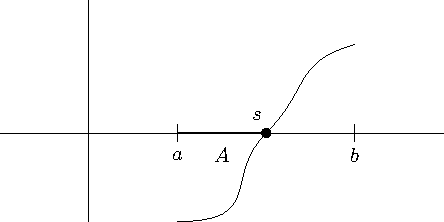
\includegraphics{images/zwischen}
  \caption{Zwischenwertsatz}%
  \label{fig:zwischen}
\end{figure}

\subsection*{Folgerungen}
\begin{zwischenwertsatz}
  Sei $f \colon [a, b] \to \mathbb{R} $
  stetig mit $f(a) \leq f(b)$.
  Dann gilt 
  \[[f(a), f(b)] \subset f([a, b]).\]
  In anderen Worten heisst das, dass stetige
  Funktionen jeden Wert zwischen
  zwei angenommenen Werten annehmen.
\end{zwischenwertsatz}

\begin{proof}
  Sei $y \in [f(a), f(b)]$. Betrachte
  auf $[a, b]$ die stetige Funktion
  $g(x) = f(x) - y$.
  Es gilt $g(a) = f(a) - y \leq 0$ und
  $g(b) = f(b) - y \geq 0$.
  Also existiert nach Theorem~\ref{thm:pre-zwischen}
  ein Punkt $p \in [a, b]$ mit $g(p) = 0$,
  beziehungsweise $f(p) = y$.
\end{proof}

\begin{example}
  Seien $a_1, a_2, \dots, a_{2k + 1} \in \mathbb{R}$.
  Setze
  \[
  f(x) = x^{2k+1} + a_1 x^{2k}
  + \cdots + a_{2k}x + a_{2k+1}.
  \]
  Dann ist $f$ ein \emph{Polynom} von ungeradem
  \emph{Grad} $2k + 1$. Es gilt
  \[
    \lim_{n \to \infty} \frac{f(n)}{n^{2k+1}}
    = \lim_{n \to \infty}
    \left( 1 + \frac{a_1}{n} + \frac{a_2}{n^2}
    + \cdots + \frac{a_{2k+1}}{n^{2k+1}}\right) = 1.
  \]
  Folglich nimmt $f$ beliebig hohe Werte an.
  Ähnlich gilt
  \[
    \lim_{n \to \infty} \frac{f(-n)}{n^{2k+1}}
    = \lim_{n \to \infty}
    \left( -1 + \frac{a_1}{n} - \frac{a_2}{n^2}
    \pm \cdots + \frac{a_{2k+1}}{n^{2k+1}}\right) = -1,
  \]
  also nimmt $f$ negative Werte
  mit beliebig hohem Betrag an.
  Nach dem Zwischenwertsatz 
  ist $f$ surjektiv, insbesondere hat $f$ eine Nullstelle.
\end{example}

\begin{remark}
  Für Polynome mit geradem Grad ist das falsch:
  Die Funktion $f(x) = x^2 + 1$ hat keine Nullstelle
  in $\mathbb{R}$.
\end{remark}

\begin{brouwer}
  Sei $f \colon [a, b] \to [a, b]$ stetig.
  Dann existiert $p \in [a, b]$ mit $f(p) = p$.
\end{brouwer}

Ein solcher Punkt $p$ mit $f(p) = p$ heisst \emph{Fixpunkt}
von $f$. Siehe auch Abbildung~\ref{fig:brouwer}.

\begin{proof}
  Betrachte die auf dem Intervall
  $[a, b]$ stetige Funktion
  $g(x) = x - f(x)$.
  Es gilt
  $
    g(a) = a - f(a) \leq 0$
    und
    $g(b) = b - f(b) \geq 0$.
  Nach dem Zwischenwertsatz existiert
  $p \in [a,b]$ mit $g(p) = 0$,
  beziehungsweise $f(p) = p$.
\end{proof}

\begin{figure}[htb]
  \centering
  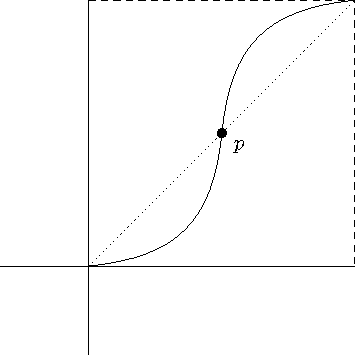
\includegraphics{images/brouwer}
  \caption{Fixpunktsatz von Brouwer.
  Ein Schnittpunkt des Graphen von $f$ mit
der Gerade mit Steigung $1$ ist ein
Fixpunkt von $f$. Die eingezeichnete Abbildung
hat sogar drei Fixpunkte, zum Beispiel $p$.}%
  \label{fig:brouwer}
\end{figure}

\section{Stetige Funktionen auf kompakten Mengen}

\begin{question}
Sei $A \subset \mathbb{R}$ beschränkt,
das heisst, es existiert $R > 0$ 
mit $A \subset [-R, R]$.
Sei $f \colon A \to \mathbb{R}$ stetig.
Ist dann $f(A) \subset \mathbb{R}$ beschränkt?
\end{question}

Die Antwort ist nein.
\begin{example}
  Sei 
  \[
    A = (0, 1) = \left\{x \in \mathbb{R} \mid 0 < x < 1\right\}
  \]
  und $f(x) = 1/x$. Dann ist $f((0, 1)) = \mathbb{R}_{>1}$ 
  unbeschränkt.
\end{example}

\begin{definition}
  Eine Teilmenge
  $U \subset \mathbb{R}$ 
  heisst \emph{offen},
  falls für
  alle $p \in U$ ein
  $\delta > 0$ existiert,
  so dass $(p - \delta, p + \delta)
  \subset U$.
Eine Teilmenge
  $A \subset \mathbb{R}$ 
  heisst  \emph{abgeschlossen},
  falls $\mathbb{R} \setminus A$ 
  offen ist.
\end{definition}

\begin{remark}
  Jede (auch unendliche) Vereinigung offener Mengen ist offen
  (aber unendliche Vereinigungen abgeschlossener Mengen
  sind nicht unbedingt abgeschlossen).
  Dazu seien $U_i \subset \mathbb{R}$ offene Teilmengen
  für $i \in I$, wobei $i$ eine 
  beliebige Indexmenge ist. Sei dann
  \[
    x \in U = \bigcup_{i \in I} U_i
  \]
  beliebig. Dann ist $x \in U_i$ für
  ein $i \in I$. Da $U_i$ offen ist, existiert
  $\delta > 0$, so dass $(x - \delta, x + \delta) \subset U_i$.
  Aber $U_i$ ist eine Teilmenge von $U$, also
  gilt auch $(x - \delta, x + \delta) \subset U$. Somit ist
  $U$ offen.
\end{remark}

\begin{examples}
  \leavevmode
  \begin{itemize}
    \item Sei
      $a < b$. Dann ist
      das \emph{offene Intervall}
      \[
        U = (a, b) = \left\{x \in \mathbb{R} \mid a < x < b\right\}
      \]
      zwischen $a$ und $b$ offen. Sei dazu $p \in (a, b)$. Setze
      $\delta = \min \{|p - a|, |p - b|\}$.
      Dann gilt
      $(p - \delta, p + \delta) \subset (a, b)$,
      siehe Abbildung~\ref{fig:offen}.
      \begin{figure}[htb]
        \centering
        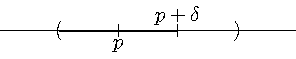
\includegraphics{images/offen}
        \caption{Offene Intervalle
        sind offen}%
        \label{fig:offen}
      \end{figure}
      
    \item Sei $a \leq b$. Dann ist das \emph{abgeschlossene Intervall}
      \[
        A = [a, b] = \left\{x \in \mathbb{R} \mid a \leq x \leq b\right\}
      \]
      zwischen $a$ und $b$ abgeschlossen.
      Sei dazu $p \notin [a,b]$, das heisst, entweder
      $p < a$ oder $p > b$.
      Setze $\delta = \min \{|p- a|, |p-b|\} > 0$.
      Dann gilt
      $(p - \delta, p + \delta) \cap [a, b] = \emptyset$,
      also ist $\mathbb{R} \setminus [a, b]$ offen.
    \item Im Extremfall $a = b$ enthält das Intervall
      $[a,b] = \{a\}$ genau einen Punkt. Also
      sind einelementige Mengen abgeschlossen.
    \item Sei $A = \{0\} \cup \left\{1/n \mid n \in 
      \mathbb{N}, n \geq 1\right\}$.
      Dann ist $A$ abgeschlossen, da
      \[
        \mathbb{R} \setminus A = \mathbb{R}_{<0} \cup
        \mathbb{R}_{>1} \cup \bigcup_{n \in \mathbb{N}_{\geq 1}}
        \left(1/(n+1), 1/n\right)
      \]
      eine Vereinigung offener Mengen und somit selbst offen ist.
    \item Die Menge
      \[
        B = \left\{1/n \mid n \in \mathbb{N}, n \geq 1\right\}
      \]
      ist weder offen noch abgeschlossen.
    \item Die Menge $\mathbb{Q} \subset \mathbb{R}$ 
      ist weder offen noch abgeschlossen.
    \item Die Menge
      \[
        [0, 1) = \left\{x \in \mathbb{R} \mid 0 \leq%chktex 9
        x < 1\right\}
      \]
      ist weder offen noch abgeschlossen.
  \end{itemize}
\end{examples}

\begin{theorem}\label{thm:extreme}
  Sei $A \subset \mathbb{R}$ nicht leer, abgeschlossen
  und beschränkt,
  und sei weiterhin $f \colon A \to \mathbb{R}$
  stetig. Dann nimmt $f$ auf $A$ ein
  Maximum beziehungsweise ein Minimum an,
  das heisst, es existiert $p \in A$,
  so dass für alle $q \in A$ gilt,
  dass $f(q) \leq f(p)$ beziehungsweise $f(q) \geq f(p)$.
\end{theorem}

Für den Beweis von Theorem~\ref{thm:extreme}
brauchen wir noch etwas Vorarbeit.

\begin{lemma*}[Folgenabgeschlossenheit]
  Sei $A \subset \mathbb{R}$ eine nichtleere Teilmenge.
  Dann ist $A$ genau dann abgeschlossen, wenn für
  alle konvergenten Folgen
  ${(a_{n})}_{n \in \mathbb{N}}$ mit
  $a_n \in A$ gilt, dass auch
  der Grenzwert $\lim_{n \to \infty} a_n$ in $A$ 
  liegt.
\end{lemma*}

Eine Menge $A$, 
so dass für alle konvergenten Folgen
${(a_{n})}_{n \in \mathbb{N}}$ mit
$a_n  \in A$ gilt,
dass auch $\lim_{n \to \infty}a_n$
in $A$ liegt, werden wir im Beweis
``folgenabgeschlossen'' nennen.

\begin{proof}
  Wir beweisen die Hinrichtung ``$\Rightarrow$'' durch Widerspruch.
  Sei
  \[
    p = \lim_{n \to \infty} a_n \in \mathbb{R} \setminus A.
  \]
  Da $\mathbb{R} \setminus A$ offen ist,
  existiert $\delta > 0$ mit $(p - \delta, p + \delta)
  \subset \mathbb{R} \setminus A$.
  Wähle $N \in \mathbb{N}$  so, dass für alle $n \geq N$
  gilt, dass $|a_n - p| < \delta$.
  Aber dann gilt $a_n \in (p - \delta, p + \delta)
  \subset \mathbb{R} \setminus A$,
  also $a_n \notin A$, was der Annahme, dass 
  $a \colon \mathbb{N} \to A$
  eine Folge in $A$ ist, widerspricht.

  Umgekehrt, für die Rückrichtung ``$\Leftarrow$'', sei
  $A \subset \mathbb{R}$ folgenabgeschlossen.
  Sei $p \in \mathbb{R} \setminus A$. Wir suchen
  $\delta > 0$, so dass $(p - \delta, p + \delta)
  \subset \mathbb{R} \setminus A$. Falls es kein
  solches $\delta > 0$ gibt, dann existiert zu jedem
  $n \in \mathbb{N}$ ein Punkt $a_n \in A$, so dass
  $|a_n - p| \leq 1/n$.
  Dann gilt
  \[
    \lim_{n \to \infty} a_n = p \in A,
  \]
  da $A$ folgenabgeschlossen ist. Das ist ein Widerspruch
  zu $p \in \mathbb{R} \setminus A$.
\end{proof}

\begin{remark}
  Etwas pathologisch ist die leere Menge $\emptyset$
  offen und somit $\mathbb{R}$ selbst abgeschlossen.
  Ausserdem ist $\mathbb{R}$ offen (da $\mathbb{R}$
  jedes Intervall enthält) und somit $\emptyset$ 
  abgeschlossen.

  Es stellt sich heraus, dass $\mathbb{R}$ und $\emptyset$ 
  die einzigen Teilmengen von $\mathbb{R}$ sind, welche
  sowohl offen als auch abgeschlossen sind.
  Äquivalent dazu ist, dass keine abgeschlossenen
  nicht-leeren Mengen $A, B \subset \mathbb{R}$ existieren,
  so dass $A \cap B = \emptyset$ und
  $A \cup B = \mathbb{R}$.
  Andernfalls könnten wir konvergente Folgen
  ${(a_{n})}_{n \in \mathbb{N}}$ in $A$
  und ${(b_{n})}_{n \in \mathbb{N}}$ in $B$ 
  konstruieren, so dass
  \[
    \lim_{n \to \infty} a_n = \lim_{n \to \infty} b_n.
  \]
  Eine Art solche Folgen zu produzieren ist folgendermassen.
  Wähle beliebige $a_0 \in A$ und $b_0 \in B$.
  Nach Konstruieren von $a_n$ und $b_n$ betrachte
  den Mittelpunkt $c_n = (a_n + b_n)/2$ und unterscheide
  zwei Fälle. Falls $c_n \in A$, setze $a_{n+1} = c_n$ 
  und $b_{n+1} = b_n$. Ansonsten, falls $c_n \in B$, setze
  $a_{n+1} = a_n$ und $b_{n+1} = c_n$.
  Die Folgen ${(a_{n})}_{n \in \mathbb{N}}$ und
  ${(b_{n})}_{n \in \mathbb{N}}$ erfüllen dann
  die gewünschte Eigenschaft. Das ist aber ein
  Widerspruch zum Lemma oben: Der gemeinsame Grenzwert
  \[
    c = \lim_{n \to \infty} a_n = \lim_{n \to \infty} b_n
  \]
  liegt nach dem Lemma oben in $A \cap B = \emptyset$.
\end{remark}

\begin{proof}[Beweis von Theorem~\ref{thm:extreme}]
  Sei $A \subset \mathbb{R}$ abgeschlossen
  und $f \colon A \to \mathbb{R}$ stetig.
  Wir beweisen in zwei Schritten, dass $f$
  ein Maximum annimmt.
  \begin{enumerate}[(i)]
    \item Die Menge $f(A) \subset \mathbb{R}$ ist 
      nach oben beschränkt.
      Andernfalls gibt es zu jedem $n \in \mathbb{N}$ 
      ein $a_n \in A$ mit $f(a_n) \geq n$.
      Da $A$ beschränkt ist, hat
      die Folge ${(a_{n})}_{n \in \mathbb{N}}$ eine
      konvergente Teilfolge
      ${(a_{n_k})}_{k \in \mathbb{N}}$ mit
      Grenzwert $p \in \mathbb{R}$.
      Da $A$ abgeschlossen, also folgenabgeschlossen
      ist, gilt
      \[
        p = \lim_{k \to \infty}a_{n_k} \in A.
      \]
      Weiter ist $f$ stetig, also folgenstetig
      in $p$, also gilt
      \[
        f(p) = \lim_{k \to \infty} f(a_{n_k})
        \geq \lim_{k \to \infty} n_k = +\infty,
      \]
      was ein Widerspruch zu $+\infty \notin \mathbb{R}$ ist.
    \item Die Funktion $f$ nimmt ein Maximum an.
      Setze $
        M = \sup \left\{f(x) \mid x \in A\right\} \in \mathbb{R}
        $.
      Es ist bloss zu zeigen, dass $p \in A$ existiert,
      so dass $f(p) = M$.
      Für alle $n \in \mathbb{N}_{\geq 1}$ existiert
      $a_n \in A$ mit $f(a_n) \geq M - 1/n$.
      Da $A$ beschränkt und abgeschlossen ist,
      hat die Folge
      ${(a_{n})}_{n \in \mathbb{N}}$ wie im
      ersten Schritt eine konvergente
      Teilfolge ${(a_{n_k})}_{k \in \mathbb{N}}$ mit
      \[
        \lim_{k \to \infty} a_{n_k}= p \in A.
      \]
      Bemerke, dass
      \[
        M - 1/n_k \leq f(a_{n_k}) \leq M.
      \]
      Da $f$ stetig, also folgenstetig in $p$ ist, folgt
      \[
        M = \lim_{k \to \infty} f(a_{n_k}) = f(p).
      \]
  \end{enumerate}
  Um zu zeigen, dass $f$ auch ein Minimum annimmt,
  bemerke lediglich, dass $-f$ ein Maximum annimmt.
\end{proof}

\begin{definition}
  Eine Teilmenge $K \subset \mathbb{R}$ heisst
  \emph{kompakt}, falls $K$ 
  beschränkt und abgeschlossen ist.
\end{definition}

\newpage
\begin{examples}
  \leavevmode
  \begin{itemize}
    \item $K = [0, 1]$ ist kompakt.
    \item Die Menge
      $
        K = \{0\} \cup \left\{1/n \mid n \in \mathbb{N}_{\geq 1}\right\} 
        \subset [0, 1]
      $
      ist kompakt.
    \item 
      Betrachte die \emph{Cantormenge}
      \[
        K = [0, 1] \setminus \bigcup_{n=1}^{\infty} U_n,
      \]
      wobei
      \begin{itemize}
        \item $U_1 = (1/3, 2/3)$,
        \item $U_2 = (1/9, 2/9) \cup (7/9, 8/9)$,
        \item $U_3 = (1/27, 2/27) \cup (7/27, 8/27) \cup (19/27, 20/27) \cup (25/27, 26/27)$,
      \end{itemize}
      und so weiter,
      siehe Abbildung~\ref{fig:cantor}.

      \begin{figure}[htb]
        \centering
        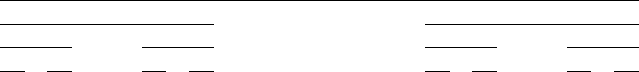
\includegraphics{images/cantor}
        \caption{Iterative Konstruktion der
        Cantormenge. Die erste Zeile ist
        $[0, 1]$, die zweite ist
        $[0, 1] \setminus U_1$, die dritte ist
        $[0, 1] \setminus (U_1 \cup U_2)$ und die
        vierte ist $[0, 1] \setminus (U_1 \cup U_2 \cup U_2)$.}%
        \label{fig:cantor}
      \end{figure}

      Offensichtlich ist $K$ beschränkt.
      Alle $U_n$ sind offen, also auch
      die Vereinigung $\bigcup_{n \in \mathbb{N}} U_n$.
      Somit ist $K$ abgeschlossen, also kompakt.
      Eine lustige Tatsache ist,
      dass Elemente von $K$ mit einem Weg
      in einem unendlich
      verzweigten binären Baum kodiert werden können,
      siehe Abbildung~\ref{fig:tree}:
      Die Menge $K$ steht in einer Natürlichen
      Bijektion zur Menge ${\{0, 1\}}^{\mathbb{N}}$,
      siehe auch den Beweis von 
      Proposition~\ref{prop:real-uncountable}
      aus Kapitel~\ref{chp:real}.
      Dort haben wir diese Bijektion explizit konstruiert.
      Das zeigt, dass die Cantormenge überabzählbar ist.

      \begin{figure}[htb]
        \centering
        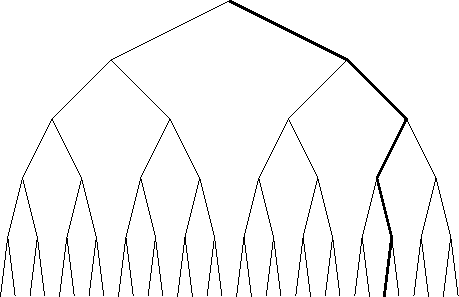
\includegraphics{images/tree}
        \caption{Ein Weg $(1,1,0,1,0, \dots)$ in einem unendlich
        verzweigten Baum}%
        \label{fig:tree}
      \end{figure}
  \end{itemize}
\end{examples}

\section{Kompakte Mengen}
\begin{proposition}[Folgenkompaktheit]
  Eine Teilmenge $K \subset \mathbb{R}$ ist
  kompakt, genau dann, wenn jede Folge
  ${(a_{n})}_{n \in \mathbb{N}}$ in $K$
  eine konvergente Teilfolge mit Grenzwert
  in $K$ besitzt.
\end{proposition}

\begin{proof}
  Für die Hinrichtung ``$\Rightarrow$''
  sei $K$ kompakt und ${(a_{n})}_{n \in \mathbb{N}}$
  eine Folge
  in $K$.
  Da $K$ beschränkt ist, hat ${(a_{n})}_{n \in \mathbb{N}}$ 
  eine in $\mathbb{R}$ konvergente
  Teilfolge  ${(a_{n_{k}})}_{k \in \mathbb{N}}$, und
  da $K$ abgeschlossen ist, liegt
  der Grenzwert $\lim_{k \to \infty} a_{n_k}$ in $K$.

  Umgekehrt, für die Rückrichtung ``$\Leftarrow$'',
  nimm an, dass $K$ folgenkompakt ist. % Nimm = Imperativ, 'man nehme' Konjunktiv I.
  Wir zeigen in zwei Schritten, dass
  $K$ kompakt ist.
  \begin{enumerate}[(i)]
    \item $K$ ist beschränkt.
      Ansonsten gibt es $a_n \in K$
      mit $|a_{n}| \geq n$.
      Aber dann hat die Folge
      ${(a_{n})}_{n \in \mathbb{N}}$ 
      in $K$ keine konvergente Teilfolge.
    \item $K$ ist abgeschlossen.
      Sei $p \in \mathbb{R} \setminus K$.
      Gesucht ist ein $\delta > 0$ 
      so dass
      $(p - \delta, p + \delta) \subset \mathbb{R} \setminus K$.
      Falls es kein solches Intervall gibt,
      dann existiert $a_n \in K$ mit
      $|a_n - p| \leq 1/n$.
      Dann ist ${(a_{n})}_{n \in \mathbb{N}}$ eine
      konvergente Folge in $K$ mit Grenzwert $p$, also gilt
      \[
        \lim_{n \to \infty} a_n = p \in K,
      \]
      da jede Teilfolge von ${(a_{n})}_{n \in \mathbb{N}}$ 
      mit Grenzwert $p$ konvergiert. Das widerspricht
      aber $p \in \mathbb{R} \setminus K$. \qedhere
  \end{enumerate}
\end{proof}

\begin{proposition}\label{prop:image-compact-compact}
  Sei $K \subset \mathbb{R}$ kompakt und
  $f \colon K \to \mathbb{R}$ stetig.
  Dann ist $f(K) \subset \mathbb{R}$ kompakt.
\end{proposition}

\begin{remark}
  Die Aussage, dass stetige Bilder kompakter Mengen
  kompakt sind, ist in vielen Gebieten der Mathematik
  enorm
  wichtig. Sie ist erstaunlich, da
  zum Beispiel stetige Bilder offener Mengen
  nicht offen sein müssen
  und ebenso brauchen stetige Bilder abgeschlossener Mengen
  nicht abgeschlossen zu sein.
  Beispiele hier sind die konstante Funktion
  $x \mapsto 0$,
  denn das Bild von $\mathbb{R}$ ist $\{0\}$,
  was nicht offen ist,
  und $\exp \colon \mathbb{R} \to \mathbb{R}$,
  denn $\exp( \mathbb{R} ) = \mathbb{R}_{>0}$
  ist nicht abgeschlossen.
\end{remark}

\begin{proof}[Beweis von Proposition~\ref{prop:image-compact-compact}]
  Auch diese Proposition zeigen wir in zwei Schritten.
  \begin{enumerate}[(i)]
    \item $f(K) \subset \mathbb{R}$ ist beschränkt.
      Das folgt aus Theorem~\ref{thm:extreme},
      welches besagt,
      dass $f$ ein Maximum und ein Minimum annimmt.
    \item $f(K)$ ist abgeschlossen.
      Sei ${(y_{n})}_{n \in \mathbb{N}}$ eine
      Folge in $f(K)$, welche mit
      Grenzwert $y \in \mathbb{R}$ konvergiert.
      Wähle
      $x_n \in K$ mit $f(x_n) = y_n$.
      Da $K$ kompakt ist,
      hat ${(x_{n})}_{n \in \mathbb{N}}$ eine
      konvergente Teilfolge
      ${(x_{n_{k}})}_{k \in \mathbb{N}}$ 
      mit Grenzwert $p \in K$.
      Da $f$ stetig, also folgenstetig in $p$ ist,
      folgt
      \[
        y = \lim_{k \to \infty} y_{n_k} 
        = \lim_{k \to \infty} f(x_{n_k}) = f(p).
      \]
      Da $f(p) \in f(K)$ gilt, folgt also,
      dass $f(K)$ folgenabgeschlossen, also abgeschlossen
      ist. \qedhere
  \end{enumerate}
\end{proof}

\subsection*{Gleichmässige Stetigkeit}
\begin{definition}
  Sei $A \subset \mathbb{R}$ beliebig.
  Eine Funktion $f \colon A \to \mathbb{R}$ 
  heisst \emph{gleichmässig stetig},
  falls für alle $\varepsilon > 0$ 
  ein $\delta > 0$ 
  existiert, so dass für alle $p, q \in A$ 
  mit $|p - q| \leq \delta$ gilt,
  dass $|f(p) - f(q)| \leq \varepsilon$.
\end{definition}

\begin{remark}
  Das unterscheidet sich von der Definition
  der Stetigkeit in einem Detail:
  Bei der gleichmässigen Stetigkeit
  darf $\delta$ nicht vom Punkt $p$ abhängen,
  was bei der herkömmlichen Stetigkeit
  erlaubt ist.
  Gleichmässige Stetigkeit impliziert
  also Stetigkeit in allen Punkten von $A$.
  Die Umkehrung gilt aber nicht.
\end{remark}

\begin{example}
  Betrachte die Funktion
  \begin{align*}
    f \colon \mathbb{R} & \to \mathbb{R} \\
    x & \mapsto x^2.
  \end{align*}
  Sei $\varepsilon > 0$ beliebig,
  zum Beispiel $\varepsilon = 1$, und $\delta > 0$ vorgegeben.  
  Sei $x > 0$ und berechne
  \begin{align*}
    f\left(x + \frac{1}{n}\right) 
    & = {\left(x + \frac{1}{n}\right)}^2 \\
               & = x^2 + \frac{2x}{n} + \frac{1}{n^2} \\
               & > f(x) + \frac{2x}{n}.
  \end{align*}
  Insbesondere gilt
  \[
  f\left(n \varepsilon + \frac{1}{n}\right)
  > f(n \varepsilon) + 2 \varepsilon
  \]
  für $n \in \mathbb{N}$. Wähle
  $n$ so, dass $1/n \leq \delta$.
  Setze $q = n\varepsilon + 1/n$ 
  und $p = n\varepsilon$.
  Dann gilt $|q - p| = 1/n \leq \delta$,
  aber
  $|f(q) - f(p)| > 2 \varepsilon > \varepsilon$.
  Also ist $f$ nicht gleichmässig stetig.
\end{example}

\begin{proposition}
  Sei $K \subset \mathbb{R}$ kompakt
  und $f \colon K \to \mathbb{R}$ stetig.
  Dann ist $f$ gleichmässig stetig.
\end{proposition}

\begin{proof}
  Wir beweisen die Proposition durch Widerspruch.
  Nimm an, dass $f \colon K \to \mathbb{R}$ nicht
  gleichmässig stetig ist.
  Dann existiert ein $\varepsilon > 0$,
  so dass für alle $n \in \mathbb{N}$ 
  ein $p_n \in K$ und ein $q_n \in K$ mit
  $|p_n - q_n| \leq 1/n$ existiert
  mit $
    |f(p_n) - f(q_n)| > \varepsilon$.
  Da $K$ kompakt ist,
  hat die Folge ${(p_{n})}_{n \in \mathbb{N}}$ 
  eine konvergente Teilfolge
  ${(p_{n_k})}_{k \in \mathbb{N}}$ 
  mit
  \[
    p = \lim_{k \to \infty}p_{n_k} \in K.
  \]
  Aus
  \[
    |p_{n_k} - q_{n_k}| \leq 1/n_k \leq 1/k
  \]
  folgt, dass
  $
    \lim_{k \to \infty} q_{n_k} = p
    $.
  Da $f$ stetig in $p$ ist, folgt, dass
  \[
    \lim_{k \to \infty} f(p_{n_k}) 
    = f(p) 
    = \lim_{k \to \infty} f(q_{n_k}).
  \]
  Das widerspricht aber der Forderung,
  dass $|f(p_{n_k}) - f(q_{n_k})| > \varepsilon > 0$.
\end{proof}

\subsection*{Topologische Charakterisierung
der Kompaktheit}
Wir erinnern uns, dass eine Teilmenge
$U \subset \mathbb{R}$ offen ist,
falls für alle
$p \in U$ ein $\delta > 0$ existiert,
so dass der $\textit{Ball}$ 
$B_p(\delta) = (p- \delta, p + \delta)$
noch ganz in $U$ liegt.

\begin{remark}
  Die offenen Teilmengen von $\mathbb{R}$ 
  erfüllen die folgenden Axiome
  eines topologischen Raums (was
  erst später im Studium relevant wird).
  \begin{enumerate}[(i)]
    \item Beliebige Vereinigungen
      offener Mengen sind offen.
    \item Endliche Schnitte offener
      Mengen sind offen.
    \item Die leere Menge und $\mathbb{R}$ selbst
      sind offen.
  \end{enumerate}
\end{remark}

\begin{warning}
  Beliebige Schnitte offener Mengen sind
  im allgemeinen
  nicht offen. 
\end{warning}

\begin{example}
  Der Schnitt
  \[
    \bigcap_{n \in \mathbb{N}} (-1/n, 1/n) = \{0\}
  \]
  ist nicht offen in $\mathbb{R}$.
\end{example}

\begin{definition}
Sei $X \subset \mathbb{R}$ eine
Teilmenge von $\mathbb{R}$.
Eine Familie ${\{U_i\}}_{i \in I}$ 
offener Mengen $U_i \subset \mathbb{R}$
heisst \emph{offene Überdeckung}
von $X$, falls
\[
  X \subset \bigcup_{i \in I} U_i,
\]
das heisst, für alle  $p \in X$ 
existiert ein $i \in I$ 
mit $p \in U_i$.
Hier ist $I$ eine
beliebige Indexmenge.
\end{definition}

In allgemeinen topologischen Räumen
ist folgendes Theorem 
die Definition der Kompaktheit.

\begin{theorem}[Heine-Borel]\label{thm:heine-borel}
  Sei $K \subset \mathbb{R}$ eine Teilmenge.
  Dann sind folgende Aussagen äquivalent.
  \begin{enumerate}[\normalfont(i)]
    \item K ist kompakt.
    \item Jede offene Überdeckung ${\{U_i\}}_{i \in I}$ 
      von $K$ enthält eine endliche offene Überdeckung,
      das heisst, es existieren
      $i_0,i_1, \dots, i_n \in I$ mit
      \[
        K \subset \bigcup_{k = 0}^n U_{i_k}
        = U_{i_0} \cup U_{i_1} \cup \cdots
        \cup U_{i_n}.
      \]
  \end{enumerate}
\end{theorem}

\newpage
\begin{examples}
  \leavevmode
  \begin{enumerate}[(1)]
    \item Sei $X = \mathbb{R}$.
      Setze
      $U_i = (i - 1, i + 1) \subset \mathbb{R}$
      für $i \in \mathbb{Z}$.
      Es gilt, dass
      \[
        X = \mathbb{R} \subset \bigcup_{i \in \mathbb{Z}} U_i,
      \]
      Für alle endlichen Teilmengen
      $M \subset \mathbb{Z}$ gilt, dass
      \[
      X \not\subset \bigcup_{i \in M} U_i.
      \]
      Also ist $X = \mathbb{R}$ nicht kompakt.
    \item Sei $K = \{0\} \cup \left\{1/n \mid 
      n \in \mathbb{N}_{\geq 1}\right\}$.
      Sei ${\{U_i\}}_{i \in I}$ eine
      beliebige offene Überdeckung von~$K$.
      Es existiert ein Index $i_0 \in I$ 
      mit $0 \in U_{i_{0}}$. 
      Da $U_{i_0} \subset \mathbb{R}$ offen ist,
      existiert $\delta > 0$ mit
      $(-\delta, \delta) \subset U_{i_0}$.
      Wähle nun $N \in \mathbb{N}$ 
      mit $1/N < \delta$.
      Dann gilt für alle $n \geq N$,
      dass $1/n \in (-\delta, \delta) \subset U_{i_0}$.
      Für alle $k \in \{1, 2, \dots, N\}$, wähle
      $i_k \in I$ mit $1/k \in U_{i_k}$.
      Dann gilt, dass
      \[
        K \subset \bigcup_{k=0}^{N} U_{i_k}
        = U_{i_0} \cup U_{i_1} \cup \cdots
        \cup U_{i_N}.
      \]
      Also enthält ${\{U_i\}}_{i \in I}$ 
      eine endliche Überdeckung von $K$.
      Folglich ist $K$ kompakt.
  \end{enumerate}
\end{examples}

\begin{proof}[Beweis von Theorem~\ref{thm:heine-borel}]
  Wir zeigen erst die Implikation
  (ii) $\Rightarrow$ (i). Sei
  ${(a_{n})}_{n \in \mathbb{N}}$ eine
  Folge in $K$. Zu zeigen ist, dass
  eine konvergente Teilfolge
  ${(a_{n_{k}})}_{k \in \mathbb{N}}$ 
  mit Grenzwert in $K$ existiert.
  Andernfalls wäre kein Punkt $p \in K$ 
  Grenzwert einer konvergenten Teilfolge.
  Dann existiert aber für jeden Punkt $p \in K$ 
  ein $\delta_p > 0$, so
  dass der Ball $B_p(\delta_p) = (p - \delta_p, p + \delta_p)$ 
  nur endlich viele Folgenglieder $a_n$ enthält.
  Präziser: nur für endlich viele $n \in \mathbb{N}$
  gilt, dass $a_n \in B_p(\delta_p)$.
  Setze  $U_p = B_{p}(\delta_p)$ für $p \in K$.
  Offensichtlich gilt
  \[
    K \subset \bigcup_{p \in K} U_p,
  \]
  also ist ${\{U_p\}}_{p \in K}$ eine offene Überdeckung
  von $K$. Nach Annahme existieren
  endlich viele $p_0, p_1, \dots, p_m \in K$ 
  mit $K \subset U_{p_0} \cup U_{p_1}
  \cup \cdots \cup U_{p_m}$.
  Nach Konstruktion enthält jede Menge~$U_{p_k}$ 
  nur endlich viele Folgenglieder
  $a_n$, also auch $K$. Das ist ein Widerspruch.
  
  Für die Richtung (i) $\Rightarrow$ (ii) seien
  $K$ kompakt und ${\{U_i\}}_{i \in I}$ eine
  offene Überdeckung von~$K$.
  Wir behaupten, dass
  $\delta_0 > 0$ existiert, so dass
  für alle $p \in K$ ein $i \in I$ existiert
  mit $B_p(\delta_0) \subset U_i$.
  Andernfalls existiert eine Folge
  ${(p_{n})}_{n \in \mathbb{N}}$ in~$K$ 
  mit folgender Eigenschaft.
  Für alle $n \in \mathbb{N}$ 
  und für alle $i \in I$ 
  gilt, dass
  $B_{p_n}(1/n) \not \subset U_i$.
  Da $K$ kompakt ist,
  existiert eine konvergente Teilfolge
  ${(p_{n_k})}_{k \in \mathbb{N}}$
   mit Grenzwert
  \[
    \lim_{k \to \infty} p_{n_k} = p \in K.
  \]
  Es existiert $i_0 \in I$ 
  mit $p \in U_{i_0}$.
  Es existiert sogar ein
  $\varepsilon > 0$, so dass
  $B_p(\varepsilon) \subset U_{i_0}$.
  Wähle $k \in \mathbb{N}$ mit
  $1/k < \varepsilon/2$
  und $|p - p_{n_k}| < \varepsilon/2$.
  Dann gilt
  \[
    B_{p_{n_k}}(1/n_k) \subset B_{p_{n_k}}(1/k).
    \subset B_p(1/k + \varepsilon / 2)
    \subset B_p(\varepsilon) \subset U_{i_0},
  \]
  siehe Abbildung~\ref{fig:heine-borel}.
  Das widerspricht aber
  $B_{p_{n_k}}(1/n_k) \not\subset U_{i_0}$
  und zeigt somit unsere Behauptung.

  Sei nun $\delta_0 > 0$, so dass
  für alle $p \in K$ 
  ein $i \in I$ existiert
  mit $B_p(\delta_0) \subset U_i$.
  Da $K$ kompakt, also beschränkt ist,
  existiert $R > 0$ mit \[K \subset
  [-R, R] = \left\{x \in \mathbb{R} \mid 
-R \leq x \leq R\right\}.\]
  Sei $N \in \mathbb{N}$ 
  mit $N > 2R/2\delta_0$.
  Dann existieren $N$ offene Intervalle
  \[
    (a_1, b_1), \dots, (a_N, b_N) \subset \mathbb{R}
  \]
  mit $b_k - a_k = 2 \delta_0$
  und
  \[
    K \subset [-R, R] \subset \bigcup_{k=1}^{N}(a_k, b_k).
  \]
  Nach der definierenden Eigenschaft von $\delta_0$
  existiert
  für alle $k \in \{1, \dots , N \}$ 
  ein $U_{i_k}$ mit
  \[
    B_{p_k}(\delta_0) = (a_k, b_k) \subset U_{i_k}
  \]
  mit $p_k = (b_k + a_k)/2$.
  Somit gilt
  \[
    K \subset \bigcup_{k=1}^{N} (a_k, b_k) \subset
    \bigcup_{k=1}^{N} U_{i_k},
  \]
  das heisst, die Familie ${\{U_i\}}_{i \in I}$ enthält
  eine endliche Überdeckung.
\end{proof}

\begin{figure}[htb]
  \centering
  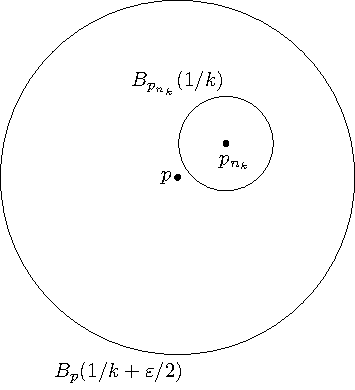
\includegraphics{images/heine-borel}
  \caption{Beweis von Theorem~\ref{thm:heine-borel}}%
  \label{fig:heine-borel}
\end{figure}


\end{document}%chktex 17
